\chapter{Cómputo distribuido}
Los flujos de trabajo requieren de recursos de cómputo para su ejecución. En los flujos de trabajo de ejemplo del capítulo \ref{chap:workflows} se mencionaron aplicaciones científicas que, por su naturaleza, requieren un alto poder de cómputo para llevarse a cabo. Por otro lado, también existen aplicaciones de negocio que, si bien son computacionalmente sencillas, se requiere ejecutar una gran cantidad de instancias de estos flujos de trabajo. Por ello, ejecutar cualquiera de estos flujos de trabajo en una sola computadora resulta prohibitivo. Por lo tanto, comúnmente se hace uso de varias computadoras para distribuir la carga computacional necesaria para correr estos procesos.

Dependiendo de cómo estén organizados estas computadoras, se definen los enfoques para correr los flujos de trabajo con cómputo distribuido.

\section{Enfoques de cómputo para flujos de trabajo}
Diversos enfoques se han aplicado para distribuir la ejecución de un flujo de trabajo entre varias computadoras.  De acuerdo a Buyya et al., los enfoques de cómputo más importantes para los flujos de trabajo son los \emph{clusters}, los \emph{grids} y las \emph{nubes} \cite{buyya2009cloud}. A continuación, explicaremos cada uno de los enfoques.

\subsection{Clusters}
Los \emph{clusters} son sistemas distribuidos, paralelos, compuestos de varias computadoras conectadas entre si que funcionan como un único recurso de cómputo \cite{buyya2009cloud}. 

Un ejemplo de un cluster se puede encontrar en la Universidad Autónoma Metropolitana, campus Iztapalapa. El cluster, llamado \emph{Aitzaloa}, está compuesto por 270 nodos de cómputo, cada uno equipado con dos procesadores Intel Xeon Quad-Core y 16GB en RAM; los nodos están conectados entre sí por medio de switches Ethernet e Infiniband. El cluster también cuenta con un sistema de archivos distribuido basado en Lustre. La capacidad real de cómputo del cluster Aitzaloa es de 18.4 teraFLOPS \cite{uamz2013tizaloa}.

El detalle de la topología del cluster se puede apreciar en la figura \ref{fig:topologia_aitzaloa}, en donde podemos apreciar que los switches son los puntos de conexión entre el nodo maestro, el sistema de almacenamiento distribuido y los nodos de cómputo.

\begin{figure}
    \begin{center}
        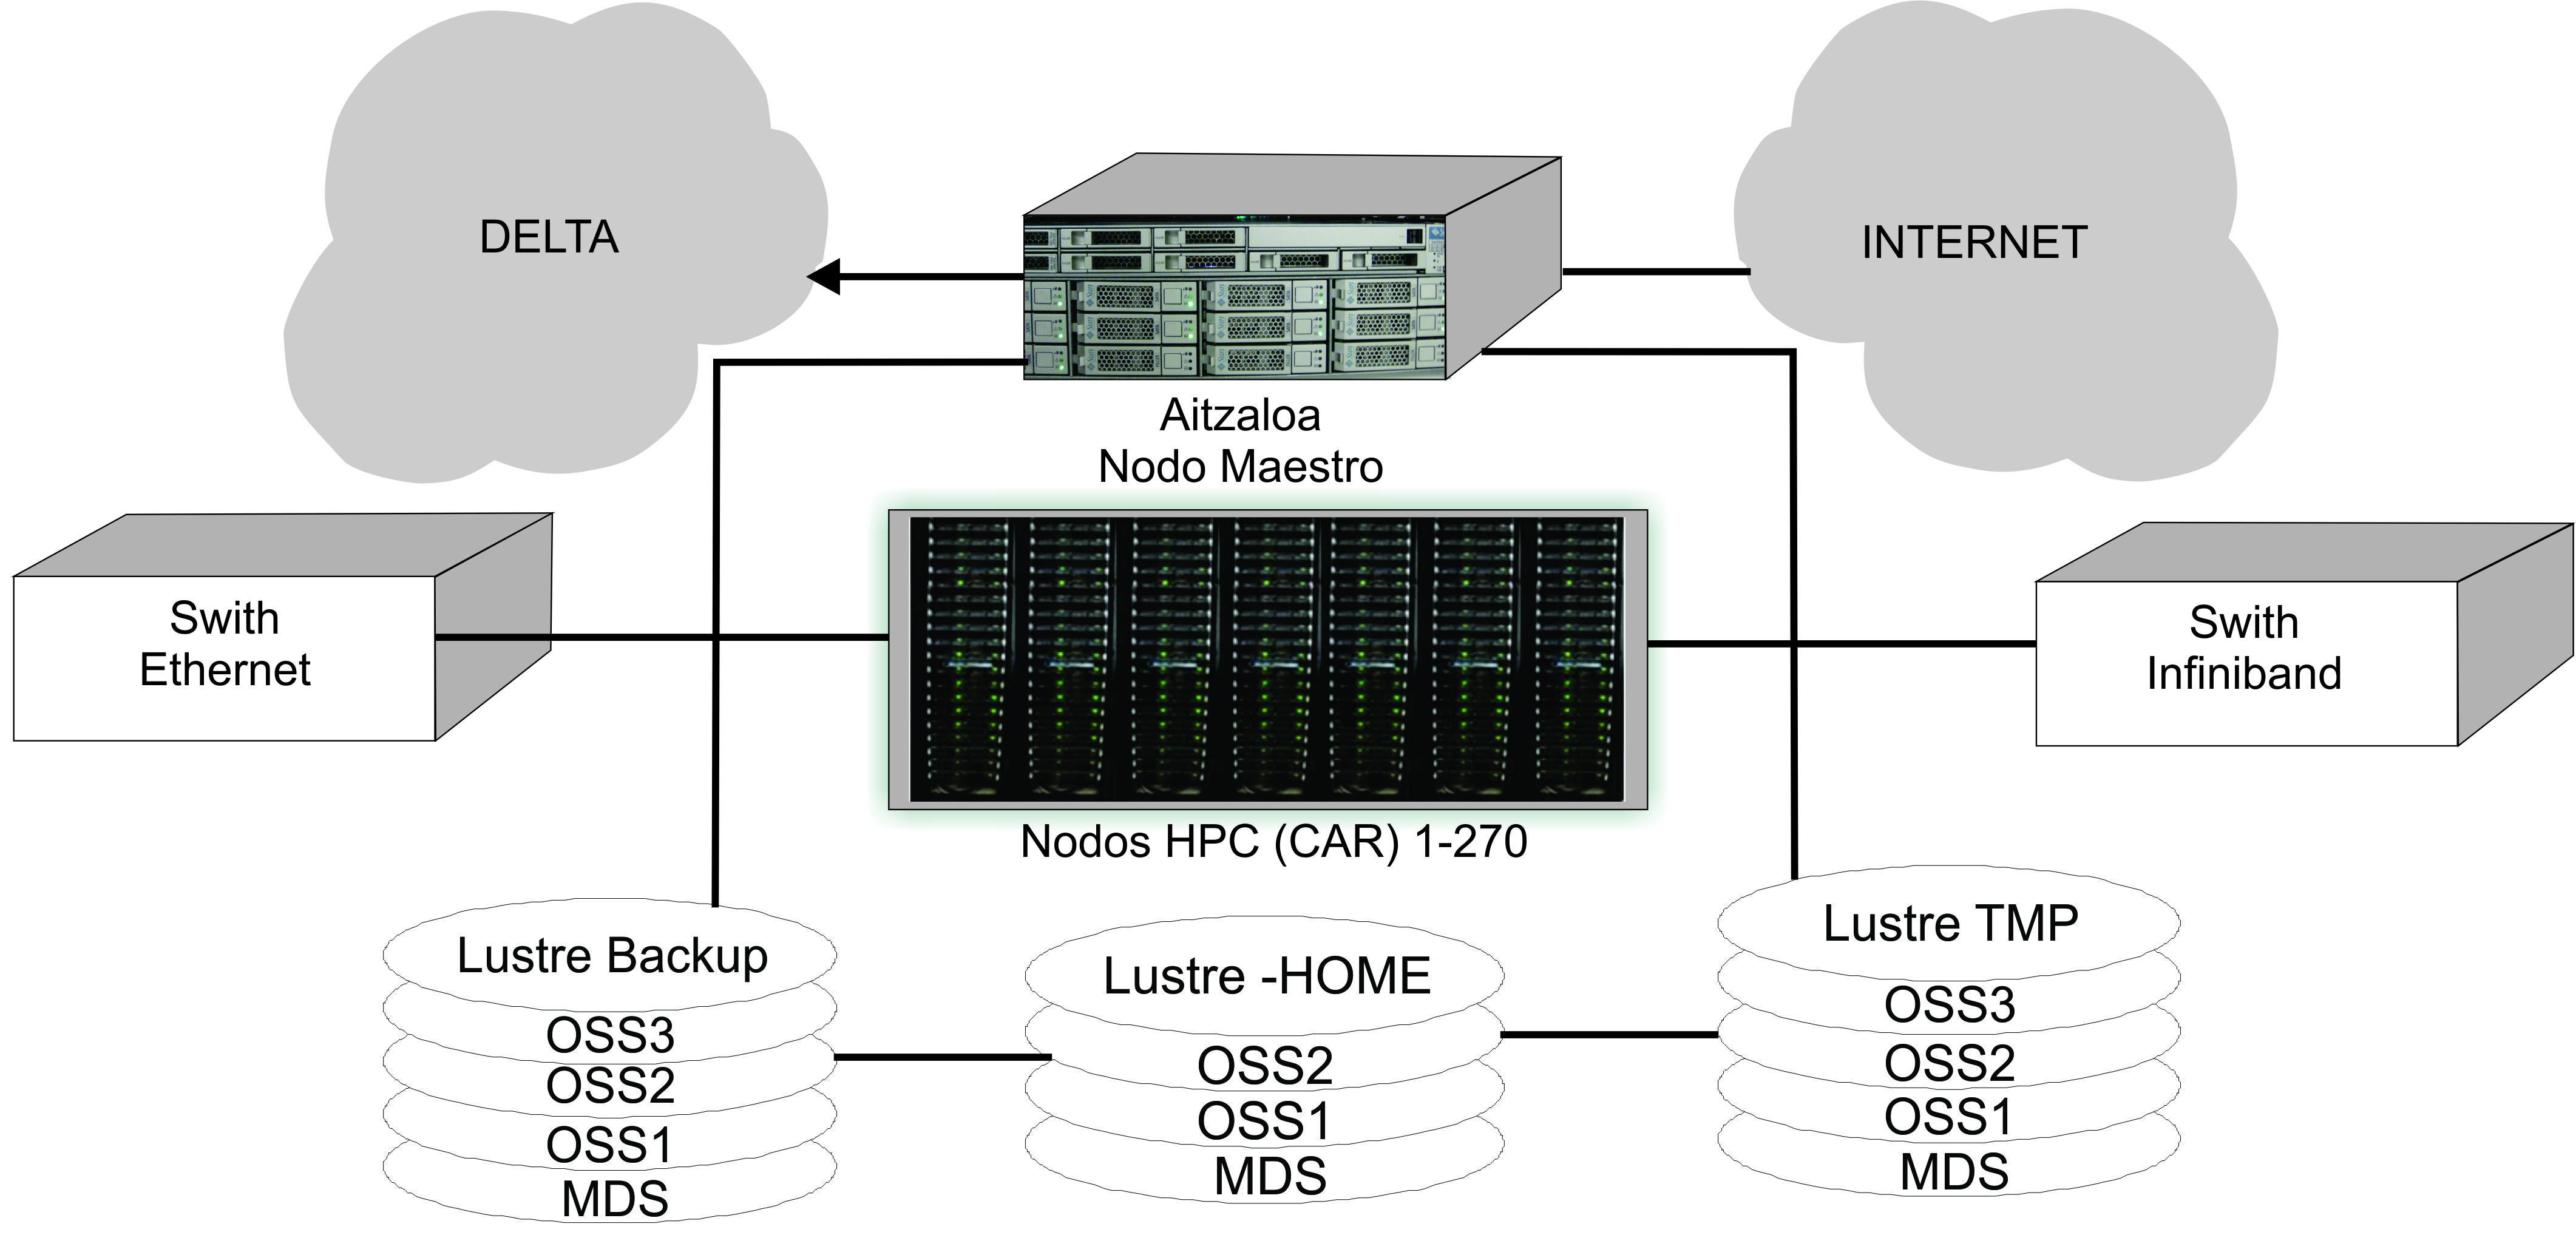
\includegraphics[width=0.8\textwidth]{imagenes/topologia_aitzaloa}
    \end{center}
    \caption{Topología del cluster Aitzaloa}
    \label{fig:topologia_aitzaloa}
\end{figure}


\subsection{Grids}
Los \emph{grids} son sistemas distribuidos, paralelos, compuestos de computadoras autónomas y geográficamente distribuidas que pueden trabajar en conjunto o de manera independiente de acuerdo a los objetivos, políticas y mecanismos de uno o varios administradores del sistema, es decir, un grid puede ser compartido entre varias instituciones \cite{buyya2009cloud}. 

El proyecto \emph{LANCAD}\footnote{Laboratorio Nacional de Cómputo de Alto Rendimiento} es un buen ejemplo, pues une el cluster \emph{Aitzaloa} de la UAM, el cluster de la UNAM \emph{KamBalam}, y el cluster \emph{Xiuhcoatl} del CINVESTAV por medio de una red de fibra óptica instalada en las estaciones del Sistema de Transporte Colectivo Metro. La suma de la potencias reales de cada \emph{nodo robusto} del grid es de 48.55 teraFLOPS \cite{lancad2013xiuhcoatl}.

En la figura \ref{fig:LANCAD-mapa-fo} se muestra los tramos de línea de Metro que cuentan con fibra óptica para conectar cada uno de las supercomputadoras (clusters) de las tres instituciones.

\begin{figure}
    \begin{center}
        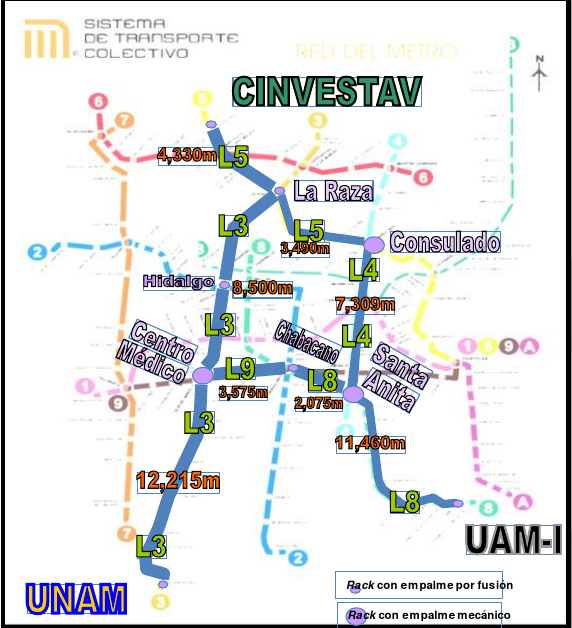
\includegraphics[width=0.8\textwidth]{imagenes/LANCAD-mapa-fo}
    \end{center}
    \caption{Red de fibra óptica del grid LANCAD.}
    %Detalle de la red de fibra óptica para conectar los nodos robustos del grid del proyecto LANCAD
    \label{fig:LANCAD-mapa-fo}
\end{figure}


\subsection{Nubes}
Las \emph{nubes} (clouds) son sistemas distribuidos, paralelos, compuestos de computadoras o máquinas virtuales interconectadas que son aprovisionadas para usarse como uno o varios recursos de cómputo, de acuerdo a un contrato de nivel de servicio acordado entre el proveedor de la nube y el cliente \cite{buyya2009cloud}. 

Empresas nuevas y existentes proveen servicios de cómputo en la nube, tales como GoGrid, Rackspace, Amazon, Microsoft, IBM, Oracle, entre otras. La forma en que operan es la siguiente: se paga cierta cantidad por utilizar servicios de cómputo o almacenamiento durante determinado tiempo. Así, los clientes no tienen que invertir grandes cantidades de dinero para contar con una gran infraestructura como en el caso de los los clusters y los grids.

\section{Comparación de los enfoques}
Si bien estos enfoques difieren, principalmente, en la forma en que están organizadas las unidades de cómputo, podemos enumerar algunas observaciones.

Primero, es natural ver que los grids están compuestos de clusters, pero también podría verse a un grid como un gran cluster. Hasta cierto punto este razonamiento parece correcto. Sin embargo, la diferencia importante entre clusters y grids radica en el hecho de que el grid es comúnmente administrado por varios técnicos de varias instituciones que, pueden tener objetivos y necesidades diversas, mientras que un cluster requiere de menos administradores y se asume una mayor flexibilidad para enfrentar fallos. \cite{buyya2009cloud} %Esta comparación viene en la primera tablita del paper%

Segundo, tanto los grids como las nubes son físicamente muy similares: ambos consisten de varios clusteres interconectados y distribuidos geográficamente. Entonces, ¿cuál es la diferencia? Lo que distingue a las nubes de los grids son dos características: (1) en una nube, se utilizan \emph{máquinas virtuales} para distribuir el recurso. El usuario tiene la vista de una parte del grid como si fuera una computadora dedicada exclusivamente para éste. Por otro lado, en los grids, es común que el usuario acceda a él con una cuenta asignada por un administrador, de tal suerte que se tiene una vista de una gran máquina que es compartida entre varios usuarios. Muchos de los administradores de grids en el mundo administran los trabajos encargados por los usuario de tal modo que se ejecuten lo más rápido posible con los recursos disponibles en un tiempo dado. Los usuarios, en algunos casos obtienen acceso al grid y trabajan sus proyectos de manera gratuita o, en caso contrario, pagan una cuota por un tiempo fijo de cómputo. Pero, en el caso de las nubes, se agrega un modelo económico para acceder a los recursos llamado \emph{pay as you go}, en donde el usuario paga una cuota por los recursos utilizados, sin alguna limitación mas que el presupuesto. Asi, el usuario podría pagar una gran cantidad para que su flujo de trabajo se ejecute en el menor tiempo posible o también podría pagar una menor cantidad sacrificando el tiempo total de ejecución del flujo.